% ================================================================
% MAIN FILE — ARTICLE MODULAR
% Compatible con tu estructura:
% sections/, figures/, references.bib, build/
% ================================================================

\documentclass[10pt,twoside]{article}

% ================================================================
% ESPACIADO COMPACTO (tu estilo)
% ================================================================

\linespread{0.95}

\setlength{\abovedisplayskip}{5pt}
\setlength{\belowdisplayskip}{5pt}
\setlength{\abovedisplayshortskip}{3pt}
\setlength{\belowdisplayshortskip}{3pt}

\renewcommand{\arraystretch}{0.85}

\setlength{\textfloatsep}{8pt}
\setlength{\floatsep}{6pt}
\setlength{\intextsep}{6pt}

\setlength{\parskip}{2pt}
\setlength{\parindent}{0pt}

% ================================================================
% GEOMETRÍA
% ================================================================

\usepackage[utf8]{inputenc}
\usepackage[a4paper,
left=1cm,
right=1cm,
top=1.5cm,
bottom=2cm,
includefoot]{geometry}

% ================================================================
% PAQUETES
% ================================================================

\usepackage{array}
\usepackage{float}
\usepackage{fancyhdr}
\usepackage{booktabs}
\usepackage{graphicx}
\usepackage{subcaption}
\usepackage{mathrsfs}
\usepackage{hyperref}

% ================= NOMENCLATURE (LISTA DE SÍMBOLOS) =================
\usepackage{nomencl}
\makenomenclature

% Ejemplos de uso en el texto:
% \\nomenclature{$T$}{Temperatura del sistema [K]}
% \\nomenclature{$u$}{Variable manipulada (entrada de control)}
% \\nomenclature{$y$}{Variable controlada (salida del sistema)}
\usepackage{tcolorbox}
\usepackage{xcolor,colortbl}
\usepackage{amsmath}
\usepackage{amssymb}
\usepackage{multirow}
\usepackage{lastpage}
\usepackage{enumitem}
\usepackage{multicol}
\usepackage{dsfont}
\usepackage{titlesec}
\usepackage{siunitx}
\usepackage{listings}
\usepackage{algorithm}
\usepackage{algorithmic}

% ================================================================
% BIBLIOGRAFÍA
% ================================================================

\usepackage[backend=biber,style=ieee]{biblatex}
\addbibresource{references.bib}

% ================================================================
% CAPTION
% ================================================================

\usepackage[labelfont=bf,labelsep=period]{caption}
\renewcommand{\figurename}{Figure}
\renewcommand{\tablename}{Table}

% ================================================================
% HEADER / FOOTER
% ================================================================

\pagestyle{fancy}
\fancyhf{}

\rhead{Proyecto}
\lhead{
\includegraphics[width=4cm,keepaspectratio]{figures/Andes.png}}

\cfoot{Page \thepage\ of \pageref{LastPage}}

\renewcommand{\headrulewidth}{0.5pt}
\renewcommand{\footrulewidth}{0.5pt}

\setlength\headheight{2.1cm}

% ================================================================
% HIPERVÍNCULOS
% ================================================================

\hypersetup{
colorlinks,
citecolor=black,
filecolor=black,
linkcolor=black,
urlcolor=black
}

% ================================================================
% COMANDOS PERSONALIZADOS
% ================================================================

\newcommand{\dev}{\dfrac{\text{d}}{\text{dt}}}
\newcommand{\dep}[1]{\frac{\partial}{\partial #1}}

\definecolor{XCOL}{RGB}{210,250,255}
\definecolor{bub}{rgb}{0.91,1.0,1.0}

\newcommand{\grad}{$^{\circ}$}

% ================================================================
% DOCUMENTO
% ================================================================

\begin{document}

{
\setlength{\parskip}{0pt}
\raggedright
{\Large\bfseries
\parbox{\linewidth}{%
Título del Proyecto
}\par
}
\vspace{0.5cm}
\normalsize
\textbf{Alvaro Paez} \par
\vspace{0.15cm}
\hrule
}

% ================================================================
% SECCIONES MODULARES
% ================================================================

\section{Introducción}

La optimización de procesos es fundamental en la industria química, debido a que constituye un factor clave para mejorar la eficiencia operativa, reducir costos y mantener una ventaja competitiva en el mercado global. Sin embargo, la búsqueda continua de un mejor rendimiento se enfrenta al desafío de gestionar procesos químicos no lineales y altamente complejos \cite{ref1, ref2}. Los sistemas industriales compuestos por múltiples equipos presentan comportamientos dinámicos complejos caracterizados por fuertes interacciones entre variables, no linealidades y acoplamientos que dificultan su análisis y control \cite{ref3, ref4}. Estas características representan un desafío significativo para los métodos de control convencionales, particularmente aquellos basados en lazos de control independientes, como los controladores PID (Proporcional–Integral–Derivativo), los cuales pueden presentar limitaciones en el manejo de dichas interacciones, así como sensibilidad a perturbaciones y efectos de retardo. Como consecuencia, pueden generarse respuestas lentas, sobreoscilaciones y dificultades para mantener la estabilidad y el desempeño óptimo del proceso. Estas características pueden generar respuestas lentas, sobreoscilaciones y dificultades para mantener la estabilidad y el desempeño óptimo del proceso.Con el fin de superar estas limitaciones, el Control Predictivo Basado en Modelo (Model Predictive Control, MPC) se ha consolidado como una de las estrategias de control avanzado más utilizadas en procesos industriales. Este método emplea un modelo dinámico del proceso para predecir su comportamiento futuro dentro de un horizonte de tiempo determinado y resolver, en cada instante de operación, un problema de optimización que permite determinar las acciones de control más adecuadas \cite{ref5}. Gracias a su capacidad para manejar sistemas multivariables, considerar restricciones operativas y anticipar el efecto de perturbaciones, el MPC ha sido ampliamente adoptado en diversos sectores industriales. No obstante, incluso las estrategias de control avanzadas, como el MPC, presentan dificultades cuando la dinámica del proceso no se conoce con precisión o está sujeta a variaciones significativas. La complejidad numérica, caracterizada por fuertes interacciones entre variables del proceso y dinámicas no modeladas, junto con la necesidad de resolver continuamente problemas de optimización, puede traducirse en respuestas insuficientes o en la falta de convergencia del controlador. Como respuesta a estas limitaciones, en los últimos años ha surgido el uso de modelos subrogados, también conocidos como metamodelos, los cuales buscan aproximar el comportamiento de modelos rigurosos mediante representaciones matemáticas más simples construidas a partir de datos \cite{ref6, ref7}. Estos modelos permiten reducir significativamente la carga computacional asociada a la simulación y optimización de procesos complejos, manteniendo al mismo tiempo un nivel adecuado de precisión en la predicción del comportamiento del sistema \cite{ref8, ref9}. El presente trabajo se enmarca en la continuidad de una línea de investigación en la cual se desarrolló previamente la subrogación de control para un proceso químico complejo con el objetivo de implementar estrategias de control predictivo orientadas al rechazo de perturbaciones en las variables del sistema \cite{ref10}. En dicho estudio se utilizó un modelo subrogado basado en representación en espacio de estados, el cual será empleado en este trabajo como referencia de comparación frente a otros métodos de identificación y modelado, específicamente los modelos ARX, ARMAX, de primer orden con tiempo muerto (FOPDT) y modelos basados en función de transferencia.


\section{Estado del arte}

La implementación de controles predictivos avanzados como el control predictivo basado en modelos (MPC) se ve 
limitada por el alto costo computacional asociado a los modelos rigurosos que describen procesos químicos complejos. 
Al requerir cálculos numéricos intensivos, la subrogación de modelos surge como una técnica eficiente para representar 
el comportamiento del sistema mediante aproximaciones matemáticas. A través de metamodelos, es posible establecer 
relaciones entre variables de entrada y salida con el objetivo de mantener la integridad del control mientras se reduce 
la carga computacional \cite{ref6}. Diversos estudios han explorado la subrogación de modelos con el propósito de 
integrarlos en sistemas de control predictivo.

\subsection{Modelos ARX y ARMAX}
Los modelos ARX (AutoRegressive with eXogenous inputs) constituyen una clase de modelos lineales de identificación de 
sistemas en tiempo discreto que describen la salida actual del sistema como una combinación lineal de sus salidas pasadas
y de las entradas actuales y pasadas \cite{ref11}. Su estructura general se expresa como:

\begin{equation}
A(q) \bar{y}(k) = B(q) \bar{u}(k-n_k) + \bar{e}(k)
\label{eq:arx_general}
\end{equation}

\begin{equation}
A(q) = a_1 + a_2q^{-1} + \cdots + a_{n} q^{-n_a}
\label{eq:arx_A}
\end{equation}

\begin{equation}
B(q) = b_1 + b_2q^{-1} + \cdots + b_{n} q^{-n_b+1}
\label{eq:arx_B}
\end{equation}

En las ecuaciones \ref{eq:arx_general} \ref{eq:arx_B}, $y(k)$ representa la salida del sistema en el instante $k$, $u(k)$ 
la entrada manipulada, $A(q)$ y $B(q)$ los polinomios que contienen los parámetros del modelo, $n_a$ y $n_b$ el número de 
polos y ceros del sistema, respectivamente, y $n_k$ el retraso del modelo. El término $e(k)$ corresponde al ruido blanco 
que captura las perturbaciones no modeladas y $q^{-1}$ es el operador de retraso. Los parámetros del modelo se estiman típicamente mediante el método de mínimos cuadrados ordinarios, lo que garantiza una 
solución analítica cerrada \cite{ref11}. Una ventaja importante de los modelos ARX en el contexto del control MPC es su 
compatibilidad directa con herramientas computacionales de identificación de sistemas, lo que permite su integración 
inmediata en esquemas de control sin necesidad de transformaciones adicionales. Estudios recientes han aplicado modelos ARX en la identificación y control de columnas de destilación, reportando  desempeños adecuados incluso cuando el proceso presenta comportamientos ligeramente no lineales \cite{ref12}. Sin embargo,  su desempeño puede verse limitado en presencia de fuertes no linealidades, situación en la que estructuras como los modelos NARX o modelos de mayor complejidad pueden ofrecer mejores resultados \cite{ref13}. No obstante, cuando el sistema presenta un nivel de ruido significativo, resulta conveniente utilizar modelos ARMAX, los
cuales incorporan un término adicional que modela explícitamente la dinámica del error:

\begin{equation}
C(q) = c_1 + c_2q^{-1} + \cdots + c_{n_c} q^{-n_c}
\label{eq:armax_C}
\end{equation}

\subsection{Representación en espacio de estados}

La representación en espacio de estados describe la dinámica de un sistema mediante un conjunto de ecuaciones diferenciales de primer orden que capturan su evolución temporal a través de un conjunto de variables internas. Estas variables se agrupan en el vector de estados, el cual contiene la información mínima necesaria para caracterizar el comportamiento dinámico del proceso y establecer la relación entre las entradas y las salidas del sistema. De manera general, esta representación se expresa mediante las ecuaciones \ref{eq:statespace_state} y \ref{eq:statespace_output}

\begin{equation}
\dot{x}(t) = A x(t) + B u(t)
\label{eq:statespace_state}
\end{equation}

\begin{equation}
y(t) = C x(t)
\label{eq:statespace_output}
\end{equation}

Donde $x(t)$ representa un vector con las derivadas de primer orden de las variables de estado, $x(t)$ es el vector de variables de estado, $u(t)$ es el vector con las variables de entrada, $y(t)$ es el vector con las variables de salida y $A$, $B$, y $C$ son las matrices de estado, entrada y salida respectivamente. Diversos estudios han aplicado esta formulación para modelar y controlar sistemas dinámicos complejos. Por ejemplo, utiliznado una representación en espacio de estados para convertir una simulación dinámica rigurosa en un modelo matemático simplificado se puede obtener la matriz de transferencia del sistema\cite{ref20}, lo que permite diseñar un controlador óptimo mediante la técnica de realimentación de ganancia, facilitando el diseño del esquema de control y mejorando el desempeño dinámico del proceso. En otra investigación se empleo el espacio de estados en la identificación de sistemas dinámicos no lineales basada en datos mediante autocodificadores profundos, un tipo de redes neuronales\cite{ref21}. En este enfoque, el autocodificador aprende una representación latente del sistema, es decir, un conjunto de variables internas no observables directamente, pero capaces de capturar la dinámica del proceso, que actúan como vectores de estado. Los autores validaron esta aproximación mediante simulaciones en lazo abierto y posteriormente evaluaron su desempeño dentro de un esquema de control predictivo basado en modelos (MPC) en lazo cerrado. Otros estudios han desarrollado un esquema de MPC para el control de procesos por lotes afectados por perturbaciones desconocidas y fallas en actuadores. En este trabajo emplearon una representación no mínima del espacio de estados, es decir, una formulación que incorpora más estados de los estrictamente necesarios para describir la dinámica de entrada–salida del proceso \cite{ref22}. Esta ampliación permitió mejorar el desempeño en el lazo cerrado, ya que el sistema logró compensar simultáneamente las variaciones en las entradas y los errores de seguimiento.

\subsection{Modelo Hammerstein--Wiener}

Los modelos Hammerstein–Wiener constituyen una estructura ampliamente utilizada para la identificación de sistemas no lineales. En este enfoque, la dinámica del proceso se describe mediante un bloque lineal formulado en espacio de estados, mientras que las variables de entrada y/o salida se transforman mediante funciones no lineales estáticas, es decir, funciones sin dinámica ni memoria. En particular, el bloque Hammerstein introduce una no linealidad estática en la entrada antes del sistema lineal, mientras que el bloque Wiener aplica una transformación no lineal a la salida del sistema lineal. Esta arquitectura permite representar comportamientos no lineales al combinar un modelo dinámico lineal, responsable de describir la evolución temporal del sistema, con transformaciones estáticas que pueden capturar fenómenos como saturaciones, zonas muertas o ganancias dependientes del estado \cite{ref23}. Debido a esta estructura híbrida, los modelos Hammerstein–Wiener resultan especialmente adecuados para procesos químicos, ya que mejoran la capacidad de representar relaciones no lineales entre las variables de entrada y salida del sistema.

\subsection{Resumen de las estrategias de subrogación}

La elección de la técnica de subrogación de modelos para el control y la optimización de procesos químicos no lineales debe basarse en las características específicas del sistema que se desea modelar. Los modelos ARX y ARMAX son adecuados cuando el proceso presenta una dinámica lineal o ligeramente no lineal, lo que permite una representación eficiente con un costo computacional bajo. Sin embargo, su aplicabilidad se ve limitada cuando el sistema presenta no linealidades complejas o perturbaciones significativas. En estos casos, las máquinas de soporte vectorial (SVM) ofrecen una mayor robustez, ya que son capaces de manejar relaciones no lineales más complejas y de generalizar bien a partir de conjuntos de datos limitados. Las SVM se convierten en una opción poderosa para sistemas con alta incertidumbre y variabilidad en sus dinámicas. A pesar de sus ventajas, su integración en esquemas de control predictivo, como el MPC, presenta desafíos debido a que los modelos no son directamente lineales y requieren técnicas adicionales para su implementación en tiempo real. Por último, la representación en espacio de estados es una opción más robusta para procesos con dinámicas altamente no lineales o para sistemas que involucran interacciones complejas entre múltiples variables. Esta técnica permite capturar de manera precisa las interacciones internas y externas del sistema, pero a costa de un mayor costo computacional, debido a la necesidad de resolver sistemas de ecuaciones diferenciales. Por todo lo anterior, se busca comparar los diferentes métodos para determinar sus diferencias en el caso propuesto. 
En la Tabla \ref{tab:comparacion_modelos} se presenta una comparación general entre las principales estrategias de modelado utilizadas en 
procesos químicos.

\begin{table}[ht]
\centering
\small
\caption{Comparación de estrategias de subrogación para control de procesos}
\label{tab:comparacion_modelos}
\renewcommand{\arraystretch}{1.3}
\setlength{\tabcolsep}{6pt}
\begin{tabularx}{\textwidth}{l l l l l X}
\hline
Modelo & Tipo & No linealidad & Complejidad & Integración MPC & Aplicaciones \\
\hline
Espacio de estados & Lineal dinámico & Baja--media & Media & Directa & Control multivariable \\
\hline
ARX / ARMAX & Lineal dinámico & Media & Media & Directa & Identificación de sistemas \\
\hline
SVM & No lineal & Alta & Alta & Requiere MPC no lineal & Sistemas no lineales \\
\hline
Hammerstein--Wiener & Híbrido & Media--alta & Media & Compatible & Procesos químicos \\
\hline
\end{tabularx}
\end{table}



\subsection{Métodos de modelamiento de columnas de destilación}

El modelamiento de columnas de destilación se basa comúnmente en el modelo MESH (Mass, Equilibrium, Summation and Heat), el cual asume 
equilibrio termodinámico entre las fases vapor y líquido en cada etapa de la columna \cite{ref10}. El número total de ecuaciones algebraicas que describen una columna de destilación en un instante dado puede calcularse mediante:

\begin{equation}
N_{ec} = N (2C + 3)
\label{eq:num_ec}
\end{equation}

donde $N$ representa el número de etapas teóricas de la columna y $C$ el número de componentes químicos presentes en el sistema. En simulaciones dinámicas, este sistema de ecuaciones se resuelve para cada intervalo de tiempo considerado en la discretización del 
proceso. Por lo tanto, el número total de ecuaciones que debe resolver el simulador se expresa como:

\begin{equation}
N_{et} = N_{ec} \times N_{i}
\label{eq:num_et}
\end{equation}

donde $N_i$ representa el número de intervalos de tiempo utilizados en la simulación dinámica. El esquema general del proceso de destilación considerado en este trabajo se presenta en el Anexo correspondiente.

\section{Metodología}

El presente trabajo se desarrolló como una extensión y comparación del estudio realizado por Quintero y Botía et al. \cite{ref10} sobre la subrogación de modelos para el control predictivo de un proceso de destilación extractiva. La metodología se estructuró en dos fases principales: $(i)$ la replicación y verificación de la base metodológica establecida en dicho trabajo, que incluye el caso de estudio, las simulaciones rigurosas y la generación de datos dinámicos; y $(ii)$ la implementación y evaluación de nuevas estrategias de subrogación orientadas al control. En la primera fase se utilizó el mismo caso de estudio correspondiente a la separación de una mezcla azeotrópica metanol-acetona mediante destilación extractiva con dimetilsulfóxido (DMSO) como agente separador. Inicialmente, se verificó el correcto funcionamiento del modelo del proceso en estado estacionario en Aspen Plus. Posteriormente, el proceso fue llevado a un entorno dinámico mediante Aspen Plus Dynamics, donde se implementó la estructura de control regulatorio necesaria para garantizar la estabilidad hidráulica del sistema durante la operación. 

Una vez estabilizado el proceso en el entorno dinámico, se realizaron pruebas de escalón en las variables manipuladas del sistema, correspondientes al calor de rehervidor y la relación de reflujo en cada columna ($Q_{R,T-101}$, $Q_{R,T-102}$, $RR_{T-101}$ y $RR_{T-102}$), mientras se monitoreó la respuesta de las variables controladas asociadas a la pureza de los productos, representadas por las temperaturas en etapas específicas de las columnas ($T_{36,T-101}$ y $T_{8,T-102})$, para obtener datos dinámicos representativos del comportamiento del sistema frente a perturbaciones.

Estos datos fueron posteriormente utilizados para la construcción de modelos subrogados capaces de aproximar el comportamiento dinámico del modelo riguroso. En el trabajo original, la subrogación del sistema se realizó mediante representaciones en espacio de estados (SS). En el presente estudio, este método de subrogación se mantiene como referencia y se implementan adicionalmente modelos ARX y ARMAX con el objetivo de comparar el desempeño de diferentes estrategias de subrogación orientadas al control. Los modelos obtenidos fueron evaluados mediante métricas estadísticas de ajuste y posteriormente integrados en un esquema de control predictivo basado en modelo (MPC) mediante una co-simulación entre Aspen Plus Dynamics y MATLAB®–Simulink®, lo que permitió analizar su desempeño frente a perturbaciones en las corrientes de alimentación del proceso.

\begin{figure}[h!]
    \centering
    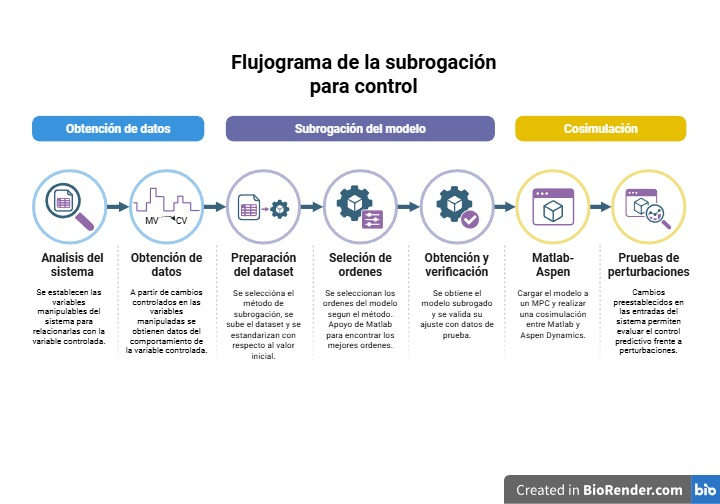
\includegraphics[width=0.6\textwidth]{figures/ProcesoControl.png}
    \caption{Flujo del proceso de subrogación de modelos para el control predictivo}
    \label{fig:ProcesoControl}
\end{figure}

\subsection{Software empleado}

Para el desarrollo de las simulaciones del proceso se empleó la suite aspenONE® de Aspen Technology Inc. (versión 11), específicamente los programas Aspen Plus V11 y Aspen Plus Dynamics V11, con el objetivo de simular el proceso tanto en estado estacionario como en régimen dinámico. Los datos generados durante la simulación dinámica fueron posteriormente exportados al entorno de MATLAB® y Simulink® R2025b de MathWorks Inc. En este entorno se realizaron las tareas de procesamiento de datos, la identificación de modelos subrogados y la implementación de los esquemas de control predictivo basados en modelo (MPC). Para la identificación de los modelos ARX y ARMAX se empleó el System Identification Toolbox de MATLAB®, el cual permite estimar modelos dinámicos a partir de datos de entrada-salida obtenidos del proceso. Por otra parte, el esquema de control MPC se implementó mediante el Model Predictive Control Toolbox, lo que permitió integrar directamente los modelos identificados en el controlador y evaluar su desempeño en el entorno de co-simulación con Aspen Plus Dynamics.



\subsection{Caso de estudio y simulación rigurosa}

Con el fin de establecer una base de comparación consistente, se adoptó el mismo caso de estudio y el modelo riguroso desarrollado por Quintero y Botía et al. \cite{ref10} correspondiente a un proceso de destilación extractiva para la separación de una mezcla azeotrópica de metanol y acetona.

\subsubsection{Descripción del proceso}

El proceso consiste en la separación de una mezcla azeotrópica de metanol-acetona mediante destilación extractiva utilizando dimetilsulfóxido (DMSO) como agente separador. La configuración del sistema está compuesta por dos columnas de destilación acopladas: una columna extractiva $T-101$ y una columna de recuperación de solvente $T-102$. En la columna extractiva $T-101$ se introduce la mezcla azeotrópica junto con el solvente DMSO, el cual modifica el equilibrio vapor-líquido del sistema y permite romper el azeótropo. Como resultado, la acetona se obtiene en el destilado mientras que la corriente de fondo contiene metanol y solvente. Esta corriente se envía posteriormente a la columna $T-102$, donde se realiza la recuperación del solvente mediante destilación, obteniéndose metanol en el destilado y DMSO en el fondo para su recirculación al proceso. El modelo del proceso se implementó inicialmente en Aspen Plus para verificar la consistencia de las condiciones operativas en estado estacionario antes de su análisis dinámico.

\subsubsection{Esquema de control regulatorio}

Para garantizar la estabilidad hidráulica y operativa del sistema durante las simulaciones dinámicas, se implementó un esquema de control regulatorio basado en controladores de retroalimentación proporcional-integral (PI). 
El sistema de control incluye lazos de control de nivel en los tanques de condensadores y rehervidores de ambas columnas, así como lazos de control de presión en cada columna de destilación. Estos lazos permiten mantener condiciones de operación estables y evitar problemas operativos tales como sobrellenado de equipos o variaciones de presión dentro del sistema. La sintonización de los controladores PI se realizó mediante el método de Tyreus-Luyben, el cual se basa en la determinación de la ganancia y el período últimos del sistema para establecer los parámetros de control adecuados. Los valores finales de sintonización corresponden a los reportados por Quintero y Botía et al. \cite{ref10}. Una vez implementado el esquema de control, se realizó una prueba de estabilidad del sistema para verificar su correcto funcionamiento. Para esta prueba se aplicó una perturbación tipo escalón correspondiente a un incremento del 15\% en el flujo molar de la corriente de alimentación azeotrópica respecto a su valor nominal. Los resultados obtenidos confirmaron que el sistema de control regulatorio permite mantener la estabilidad hidráulica del proceso, lo que constituye una base adecuada para el análisis dinámico posterior.

\subsubsection{Generación de datos dinámicos mediante pruebas de escalón}

Para obtener los datos necesarios para la identificación de modelos subrogados se realizaron pruebas de escalón (step tests) en la simulación dinámica del proceso utilizando Aspen Plus Dynamics. Estas pruebas consisten en aplicar cambios escalón en las variables manipuladas del proceso y registrar la respuesta dinámica de las variables de interés, con el propósito de excitar la dinámica del sistema y generar información suficiente para la identificación de modelos dinámicos.

En el contexto de la subrogación orientada al control, las variables manipuladas consideradas fueron la potencia de los rehervidores y la razón de reflujo de cada columna. Debido a que la medición directa de fracciones molares en procesos industriales continuos puede resultar costosa o difícil de implementar, se seleccionaron las temperaturas de etapa como variables controladas, dado que presentan una fuerte correlación con la pureza de los productos. En particular, se seleccionaron la temperatura de la etapa 36 para la columna $T-101$ y la temperatura de la etapa 8 para la columna $T-102$, debido a su alta sensibilidad frente a cambios en las condiciones operativas.

Durante el análisis de los datos obtenidos se observó la presencia de pequeñas variaciones residuales en las señales de temperatura que no son completamente explicadas por los cambios escalón aplicados. Estas variaciones pueden interpretarse como ruido en los datos, asociado principalmente aerrores de modelado y a la capacidad limitada de los modelos subrogados para reproducir completamente la dinámica del sistema, así como a efectos numéricos inherentes a la discretización temporal y a los algoritmos de integración empleados en la simulación dinámica. Este comportamiento resulta relevante para la identificación de modelos subrogados, particularmente en estructuras como los modelos ARX y ARMAX, en los cuales el término de ruido representa dinámicas no modeladas y errores de aproximación inherentes al proceso de identificación


\subsection{Subrogación de modelos}

La subrogación del proceso se realizó con el objetivo de construir modelos dinámicos simplificados capaces de reproducir el comportamiento del modelo riguroso y que puedan ser utilizados dentro de esquemas de control predictivo basado en modelo. En el trabajo original de Quintero y Botía et al. \cite{ref10}, la subrogación se realizó mediante representaciones en espacio de estados. En el presente estudio, dicho modelo se mantiene como referencia o línea base para la comparación, y se implementan adicionalmente modelos de tipo ARX y ARMAX con el fin de evaluar su capacidad para representar la dinámica del proceso.

\subsubsection{Preprocesamiento de datos}

Antes de identificar los modelos, todas las variables de entrada y salida se transformaron en desviaciones respecto a su valor nominal de operación. Esta transformación permite centrar el análisis en la dinámica del proceso alrededor del punto de operación. La desviación de cada variable se calculó mediante:

\begin{equation}
X_{desv} = \frac{(X-X_{nominal})}{X_{nominal}}
\label{eq:Desviacion}
\end{equation}

\subsubsection{Identificación de modelos subrogados}

La identificación de los modelos subrogados se realizó en el entorno MATLAB® R2025b, empleando el System Identification Toolbox, a partir de los datos obtenidos de las simulaciones dinámicas del proceso. En primer lugar, se consideró como referencia el modelo en espacio de estados desarrollado en el trabajo previo. Posteriormente, se identificaron modelos de tipo ARX y ARMAX con el objetivo de evaluar su capacidad para aproximar la dinámica del proceso mediante estructuras lineales discretas. Para los modelos ARX se llevó a cabo un barrido sistemático de órdenes utilizando las funciones arxstruc y selstruc del toolbox, las cuales permiten explorar automáticamente distintas combinaciones de parámetros autorregresivos y exógenos. En este contexto, los términos autorregresivos corresponden a valores pasados de la variable de salida del sistema (temperatura de etapa), mientras que los términos exógenos representan la influencia de las variables de entrada del proceso, en este caso la potencia del rehervidor y la razón de reflujo de cada columna. Una vez determinada la estructura ARX más adecuada, esta se utilizó como base para la identificación de modelos ARMAX, variando el orden asociado al polinomio de ruido (nc) y estimando los parámetros del modelo mediante las rutinas de identificación disponibles en el toolbox. Para cada valor de nc, se generó un modelo candidato y se evaluó su desempeño mediante simulación frente a los datos originales. El desempeño de cada modelo, para cada columna del proceso ($T-101$ y $T-102$), se evaluó mediante el coeficiente de determinación (R²) y el error cuadrático medio (RMSE) entre las salidas del modelo y los datos generados por el modelo riguroso. Estos indicadores permitieron seleccionar las estructuras con mejor capacidad predictiva para su posterior implementación en el esquema de control predictivo basado en modelo.

\subsubsection{Métricas de evaluación}

Para evaluar la capacidad de los modelos subrogados de reproducir la dinámica del proceso se emplearon métricas estadísticas de ajuste. En particular, se calcularon el coeficiente de determinación $R^2$ y  la media cuadrática del error (RECM), los cuales permiten cuantificar la calidad del ajuste entre las predicciones del modelo y los datos obtenidos de la simulación rigurosa. Las métricas se calcularon según las ecuaciones \ref{eq:RECM} y \ref{eq:R2}:

\begin{equation}
RECM= \sqrt[2]{\frac{\sum_{n=1}^N (y_n - \hat{y}_n)^2}{N}}
\label{eq:RECM}
\end{equation}

\begin{equation}
R^2 = 1 - \frac{\sum_{n=1}^N (y_n - \hat{y}_n)^2}{\sum_{n=1}^N (y_n - \bar{y})^2}
\label{eq:R2}
\end{equation}

\subsection{Implementación del control MPC y co-simulación}

Con el fin de evaluar el desempeño de los modelos subrogados dentro de un entorno de control, se implementó un esquema de MPC mediante una co-simulación entre Aspen Plus Dynamics y MATLAB®–Simulink®. En este esquema, la simulación dinámica del proceso se ejecuta en Aspen Plus Dynamics, mientras que el controlador MPC se implementa en Simulink. La comunicación entre ambos entornos permite que el controlador utilice los modelos subrogados para calcular las acciones de control en cada instante.Las variables manipuladas consideradas fueron la potencia de los rehervidores y la razón de reflujo de las columnas, mientras que las variables controladas correspondieron a las temperaturas de etapa seleccionadas para cada columna. Para evaluar el desempeño del controlador se aplicaron perturbaciones de tipo escalón en los flujos de alimentación del proceso durante un horizonte dinámico de simulación de 100 horas. El desempeño del sistema de control se evaluó en términos del error relativo respecto al valor nominal de la variable controlada, del tiempo de estabilización del sistema y del esfuerzo de control requerido para mantener la operación estable.

\subsubsection{Formulación del problema de optimización MPC}

En cada instante de control k, el controlador MPC resuelve un problema de optimización utilizando un problema de programación cuadrática (QP). Este tiene un vector de decisión $z_k$ que define la secuencia futura de acciones de control frente a las variables manipuladas:

\begin{equation}
z_k^T=[u(k|k)^T u(k+1|k)^T \cdots u(k+p-1|k)^T, \epsilon_k )]
\label{eq:Vectorzk}
\end{equation}

\begin{equation}
\min_{z_k} J(z_k) = J_y(z_k) + J_u(z_k) + J_{\Delta u}(z_k) + J_{\epsilon}(z_k)
\label{eq:OptimizationProblem}
\end{equation}
    
Dentro del vector, se optimizan dichas acciones a lo largo del horizonte de predicción p, al mismo tiempo que $\epsilon_k$ penaliza las violaciones de las restricciones. El MPC realiza la acción de la ecuación \ref{eq:OptimizationProblem}, minimizando una función de costo resultante de la suma de cuatro términos. El primer termino $J_y$, formulado en la ecuación \ref{eq:Jy}, compara el error entre las salidas propuestas por los metamodelos con su referencia a lo largo del horizonte, mientras que $J_u$, de la ecuación \ref{eq:Ju}, penaliza las desviaciones de las dos variables manipuladas con respecto al valor en estado estable. Por el otro lado, el término $J_{\Delta u}$, expuesto en la ecuación \ref{eq:Jdeltau}, compara los cambios en las variables manipuladas consecutivas para evitar cambios bruscos. Por último, $J_{\epsilon}$ penaliza la variable de relajación asociada a posibles violaciones de restricciones, garantizando que estas solo ocurran cuando sea estrictamente necesario \cite{ref24}.

\begin{equation}
J_y (z_k )=\sum_{j=1}^{n_y}\sum_{i=1}^{p}\left\{\frac{w_{i,j}^y}{s_j^y} [r_j (k+i|k)-y_j (k+i|k)]\right\}^2 
\label{eq:Jy}
\end{equation}

\begin{equation}
J_u (z_k )=\sum_{j=1}^{n_u}\sum_{i=1}^{p-1}\left\{\frac{w_{i,j}^u}{s_j^u} [u_j (k+i|k)-u_{j,target} (k+i|k)]\right\}^2
\label{eq:Ju}
\end{equation}

\begin{equation}
J_{\Delta u} (z_k )=\sum_{j=1}^{n_u}\sum_{i=1}^{p-1}\left\{\frac{w_{i,j}^{\Delta u}}{s_j^u} [u_j (k+i|k)-u_j (k+i-1|k)]\right\}^2     
\label{eq:Jdeltau}
\end{equation}

\begin{equation}
J_{\varepsilon} (z_k )=\rho_{\varepsilon} \varepsilon_k^2 
\label{eq:Jepsilon}
\end{equation}

En el contexto del estudio realizado, los modelos subrogados SS, ARX y ARMAX son los responsables del cálculo de las salidas predichas y   $(k+i|k)$, además de proporcionar la relación dinámica entre las variables manipuladas futuras $u(k+i|k)$ y el comportamiento esperado del proceso; permitiendo así que el optimizador evalúe el impacto de cada posible secuencia de control sobre el desempeño futuro del sistema.

\subsubsection{Integración con Aspen Plus Dynamics}

La co-simulación entre Simulink y Aspen Plus Dynamics se realiza mediante el intercambio de señales de entrada y salida en cada intervalo de muestreo, donde Aspen envía a Simulink las mediciones actuales de las variables controladas (temperaturas de etapa) y el controlador MPC calcula las acciones de control, las cuales son enviadas de regreso a Aspen como ajustes en la potencia de los rehervidores y en la razón de reflujo, permitiendo así cerrar el lazo de control y considerar de forma dinámica la influencia de perturbaciones externas en el proceso. 

\subsubsection{Evaluación del desempeño del controlador}
\label{sec:criterios}

Para cuantificar la efectividad del esquema de control implementado, se evaluó el desempeño del sistema mediante un conjunto de métricas que permiten analizar la calidad del seguimiento de referencia, la rapidez de respuesta del sistema y el esfuerzo requerido por las variables manipuladas. El error relativo de seguimiento permite cuantificar la diferencia entre el valor de la variable controlada y su valor de referencia a lo largo del tiempo. Este indicador se calcula mediante la siguiente expresión:

\begin{equation}
e_{rel}(t)= \frac{|Y(t)-Y_{ref} (t)|}{Y_{ref} (t)}
\label{eq:ErrorRelativo}
\end{equation}

El tiempo de estabilización se define como el tiempo requerido para que las variables controladas ingresen y permanezcan dentro de una banda de tolerancia de ±2\% respecto a su valor nominal después de la aplicación de una perturbación. Este indicador permite evaluar la rapidez con la que el sistema recupera condiciones estables de operación. Además, para evaluar con mayor precisión la calidad del control, se utilizaron las siguientes métricas de error integral.

El criterio de la integral del valor absoluto del error (IAE) mide el error absoluto acumulado a lo largo del tiempo y se calcula como:

\begin{equation}
\text{IAE} = \int_0^{\infty} |e(t)| \, dt
\label{eq:IAE}
\end{equation}

El criterio de la integral del error cuadrático mide el error cuadrático acumulado, penalizando los errores de mayor magnitud:

\begin{equation}
\text{ISE} = \int_0^{\infty} e^2(t) \, dt
\label{eq:ISE}
\end{equation}

Por otro lado, el criterio de la integral del valor absoluto del error multiplicado por el tiempo (ITAE) pondera los errores con el tiempo, favoreciendo la penalización de los errores que persisten durante períodos prolongados:

\begin{equation}
\text{ITAE} = \int_0^{\infty} t|e(t)| \, dt
\label{eq:ITAE}
\end{equation}

Finalmente, la integral del error cuadrático multiplicado por el tiempo (ITSE) es una métrica análoga a la ITAE, pero incorpora el error al cuadrado, lo que incrementa la penalización de los errores de mayor magnitud y duración:

\begin{equation}
\text{ITSE} = \int_0^{\infty} t e^2(t) \, dt
\label{eq:ITSE}
\end{equation}

Estas métricas de error integral permiten una evaluación más completa del desempeño del controlador, ya que cuantifican tanto la magnitud de los errores como su persistencia en el tiempo \cite{ref25}. Los resultados obtenidos con estas métricas permitieron comparar la capacidad de los distintos modelos subrogados para mantener la estabilidad del proceso, minimizar el error de seguimiento y reducir el esfuerzo de control requerido, proporcionando así una evaluación cuantitativa del desempeño de cada estrategia de modelado dentro del esquema de control predictivo basado en modelo.


\section{Resultados y Discusión}

Entre los resultados obtenidos, primero se comparó el ajuste de la subrogación del modelo con respecto a los datos del steptest. Posteriormente se realizó una evaluación del control por medio de los datos obtenidos en la co-simulación de Simulink y Aspen Plus Dynamics por métodos gráficos y los índices de rendimiento presentados anteriormente.

\subsection{Subrogación de modelos}

Los modelos subrogados se realizaron a partir de la consideración de dos entradas; la potencia del rehervidor y la relación de reflujo, con una salida de temperatura de etapa. En el caso de la $T-101$, los modelos predicen la temperatura de la etapa 36, mientras que en la $T-102$ se encuentra la temperatura de la etapa 8. Esto considerando los perfiles de temperatura donde se determina que estas etapas son las de mayor sesibilidad \cite{ref10}. De esta manera se obtienen los 4 modelos porevaluar para las dos torres: ARX, ARMAX, SS y NLARX-SVM. Se evalúan métricas de ajuste del sistema, sin embargo, un perfecto acople no es necesario para la implementación del modelo en control predictivo. En la Tabla 2 se puede evidenciar el RMSE y el R2, los cuales presentan una pequeña mejora en el siguiente orden entre modelos: $SS<ARX<ARMAX< NARX-SVM$ para $T-101$ y $ARX<ARMAX<SS< NARX-SVM$ para $T-102$. No obstante, es importante recalcar el alcance de todos los metamodelos al representar la tendencia general.

\begin{figure}[htbp]
    \centering
    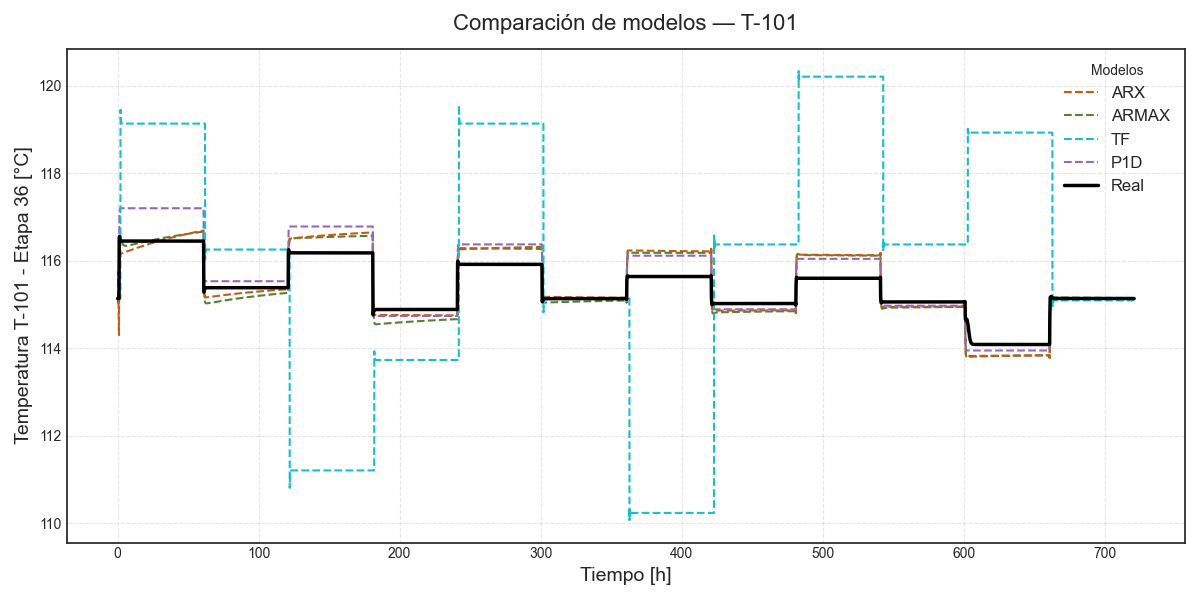
\includegraphics[width=0.6\textwidth]{figures/ModelosT101.png}
    \caption{Comparación de los modelos subrogados para el control de $T-101$}
    \label{fig:ModelosSubrogadosT101}
\end{figure}

\begin{figure}[htbp]
    \centering
    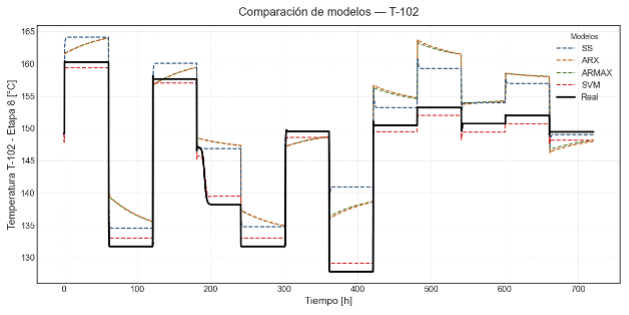
\includegraphics[width=0.6\textwidth]{figures/ModelosT102.png}
    \caption{Comparación de los modelos subrogados para el control de $T-102$}
    \label{fig:ModelosSubrogadosT102}
\end{figure}

\begin{table}[htbp]
\centering
\caption{Métricas de las subrogaciones de control}
\label{tab:ModelosR2}
\renewcommand{\arraystretch}{1.1}
\setlength{\tabcolsep}{6pt}
\begin{tabular}{l l c c}
\toprule
Columna & Modelo & RECM & $R^2$ \\
\midrule
T-101 & SS    & 1.4331 & 0.8327 \\
T-101 & ARX   & 1.4276 & 0.8340 \\
T-101 & ARMAX & 1.4073 & 0.8387 \\
T-102 & SS    & 5.4304 & 0.7232 \\
T-102 & ARX   & 5.7524 & 0.6894 \\
T-102 & ARMAX & 5.7294 & 0.6919 \\
\bottomrule
\end{tabular}
\end{table}

\FloatBarrier
\subsection{Control predictivo frente a perturbaciones}

Al obtener los modelos que relacionan las variables manipuladas con la variable controlada, es posible implementar el MPC y realizar pruebas de comportamiento frente a perturbaciones. Estas son un aumento del 8\% en ente. Teniendo en consideración la implementación de los modelos en el MPC, solo se realizó el control predictivo de los modelos lineales: ARX, ARMAX, SS. Los resultados comparativos se dividieron en tres partes, comenzando por los costos computacionales en la Tabla 4 que evalúan el tiempo de Simulink, el CPU utilizado por paso y la memoria RAM necesaria para la simulación. Comparando los tres modelos se evidencia que el costo de segundos en Simulink y milisegundos de CPU por paso es el menor para el modelo de espacio de estado, sin embargo, la memoria RAM es la mayor a comparación de los otros dos modelos. A pesar de esto, es posible observar que las diferencias entre costos computacionales no son amplias, por lo cual son necesarios más criterios para determinar el mejor modelo.


\begin{figure}[htbp]
    \centering
    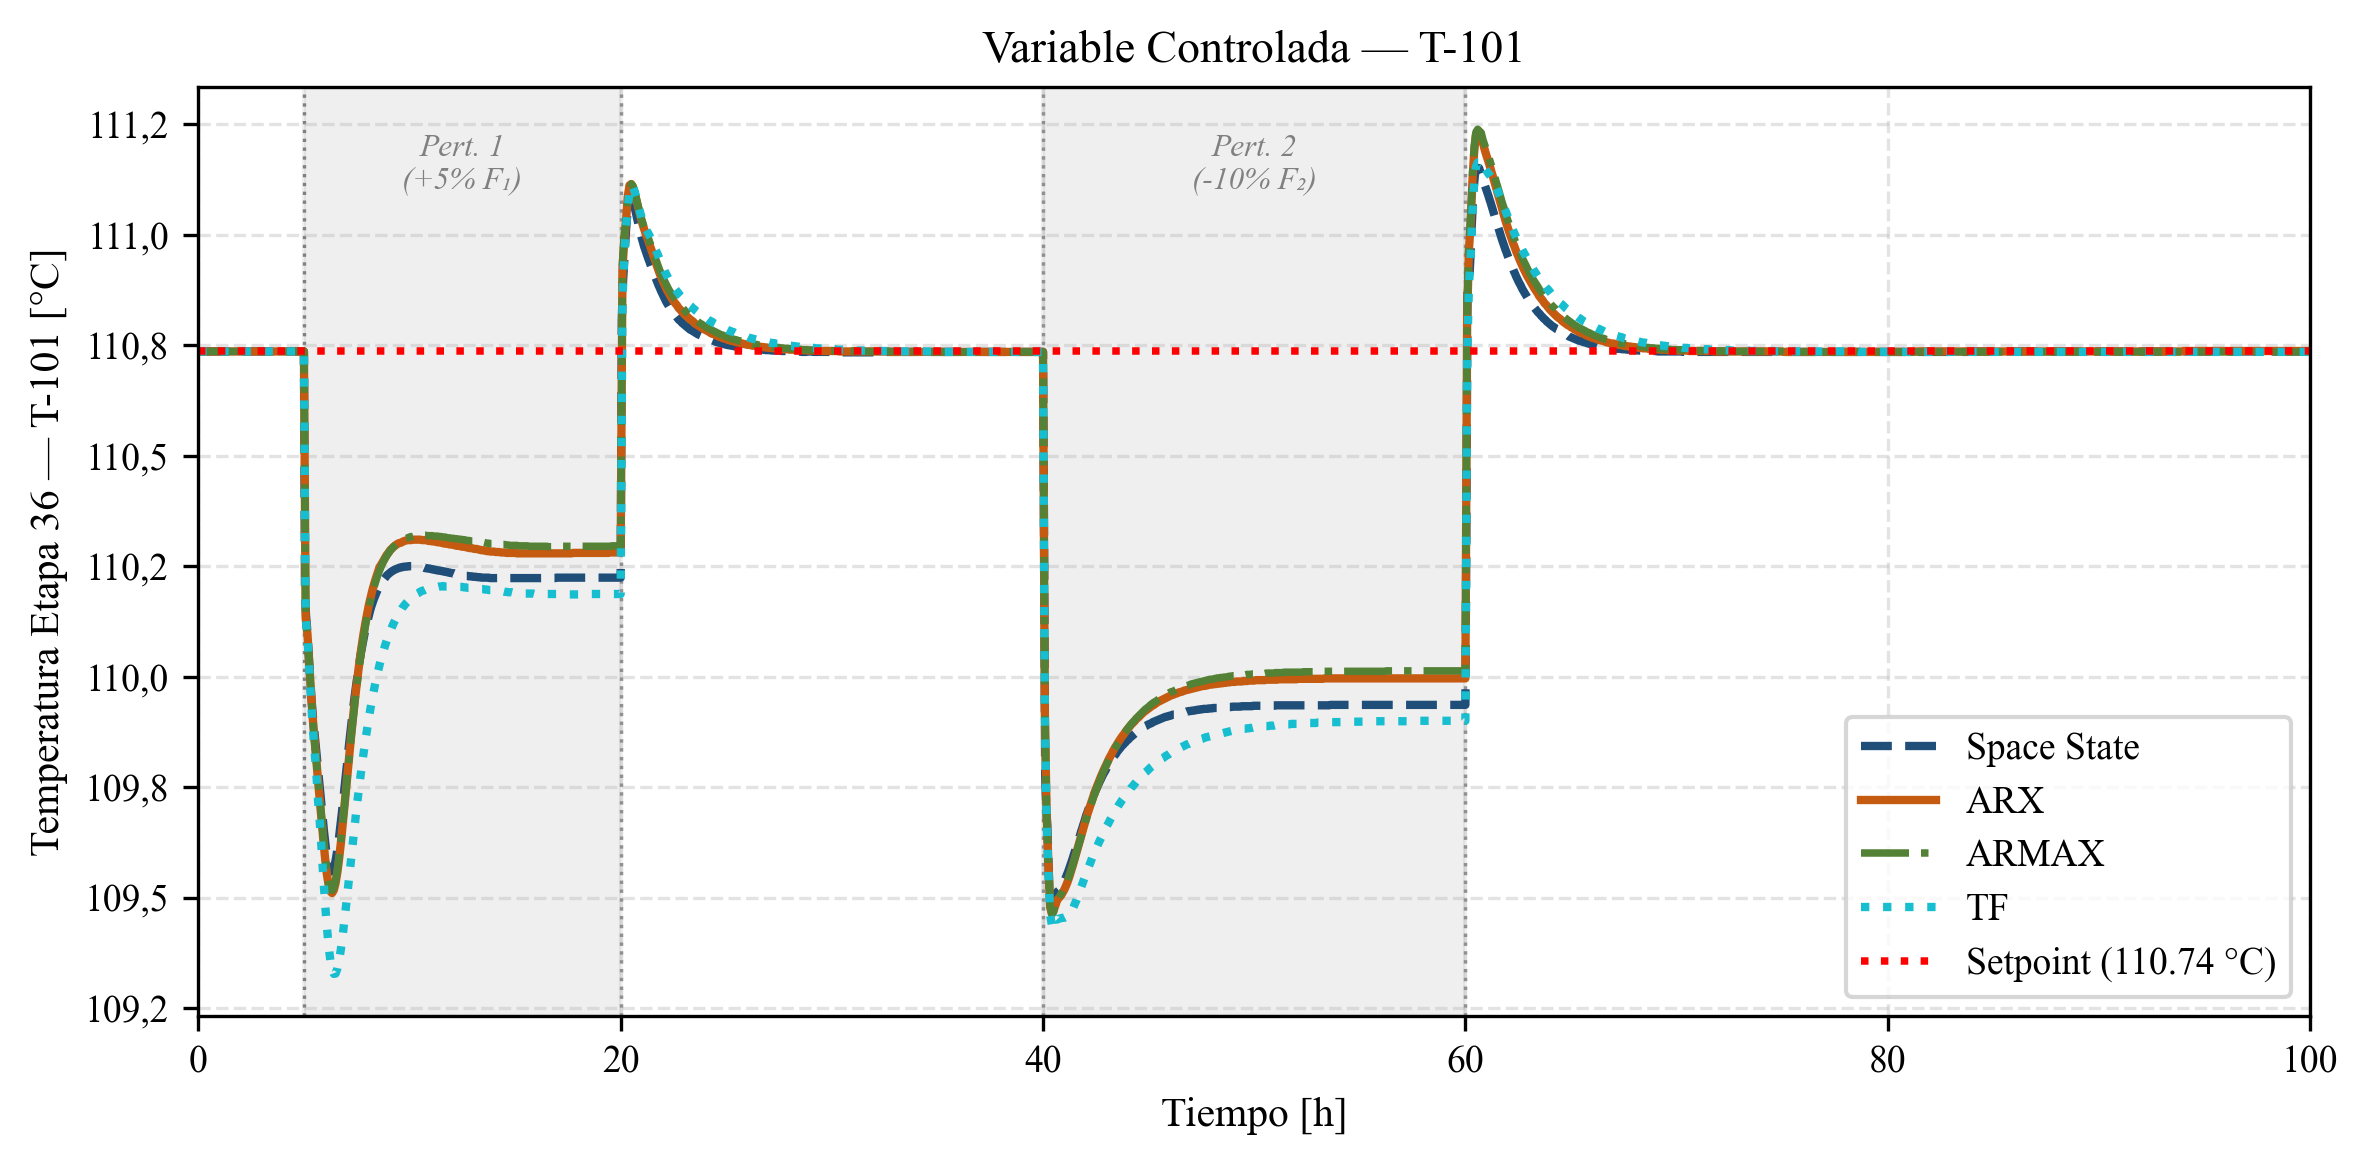
\includegraphics[width=0.6\textwidth]{figures/ControlT101.png}
    \caption{Comportamiento de la variable controlada en comparación con el valor nominal en la simulación de control $T-101$}
    \label{fig:ControlT101}
\end{figure}

\begin{figure}[htbp]
    \centering
    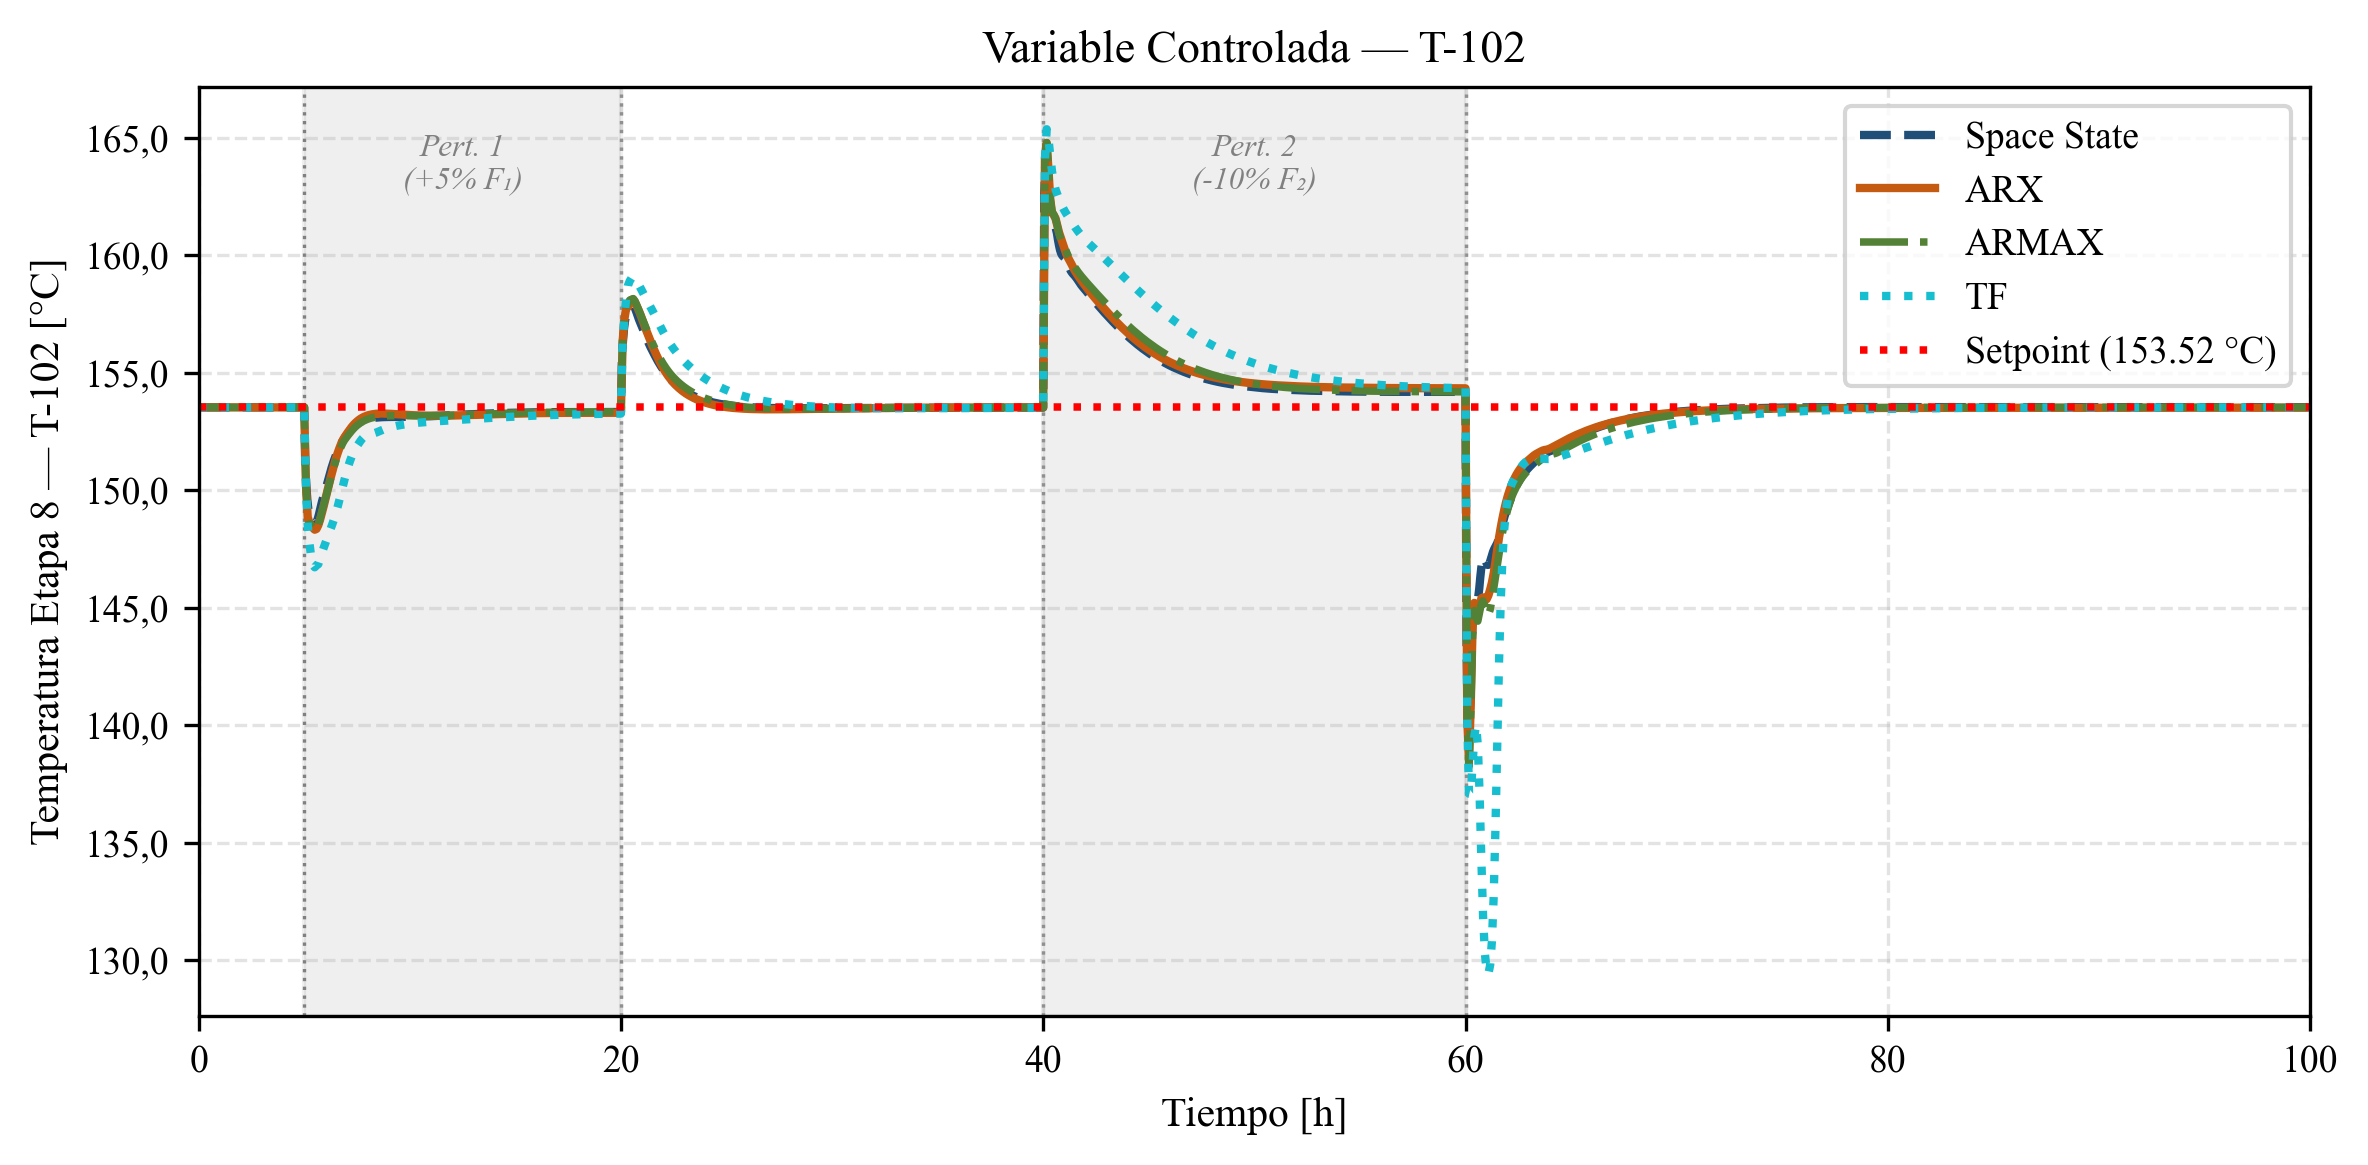
\includegraphics[width=0.6\textwidth]{figures/ControlT102.png}
    \caption{Comportamiento de la variable controlada en comparación con el valor nominal en la simulación de control $T-102$}
    \label{fig:ControlT102}
\end{figure}

Continuando con las métricas de control básicas, se comparan los tiempos de estabilización y el error con respecto al setpoint para las dos perturbaciones en cada modelo. En la Tabla 5 de denota que todos los metamodelos implementados en el MPC lograron alcanzar un error menor al 1\%, por lo que el objetivo de control de perturbaciones se alcanzó en los tres casos. De todos modos, se puede visualizar tanto en la tabla como en la Figura 4 y Figura 5 existen diferencias en el error y el tiempo de estabilización. En general, el modelo ARMAX generó una estabilización más rápida, de 6.7 horas aproximadamente, cercana a valores de literatura a comparación de los otros dos modelos. Sin embargo, el error en este metamodelo aumenta; caso contrario al modelo ARX, el cual tiene los errores más pequeños; incluso llegando a 0.2\% en $T-102$ para la primera perturbación; pero aumentando considerablemente el tiempo de estabilización. Debido a que ningún modelo es concluyente al compararlos por medio del tiempo y el error, es necesario utilizar criterios integrales de desempeño para determinar cuál realiza el mejor trabajo de control.

\begin{table}[htbp]
\centering
\caption{Costos computacionales}
\label{tab:CostosComputacionales}
\small
\begin{tabular}{lccc}
\toprule
Modelo & T. Simulink (s) & CPU/paso (ms) & RAM (MB) \\
\midrule
SS    & 1373.914 & 1136.406 & 6.156  \\
ARX   & 1425.248 & 1178.865 & 5.9959 \\
ARMAX & 1463.379 & 1210.405 & 6.0456 \\
\bottomrule
\end{tabular}
\end{table}

\begin{table}[htbp]
\centering
\caption{Métricas de las subrogaciones de control}
\label{tab:ControlMetrics}
\scriptsize
\setlength{\tabcolsep}{3pt}
\begin{tabular}{llcccccccc}
\toprule
Sistema & Modelo & P1 [°C] & P2 [°C] & SP [°C] & $er_1$ & $er_2$ & $t_1$ [h] & $t_2$ [h] \\
\midrule
T-101 & SS    & 109.93  & 110.19  & 110.73 & 0.72 & 0.49 & 7.42 & 6.42 \\
T-101 & ARMAX & 109.858 & 110.134 & 110.73 & 0.79 & 0.54 & 6.66 & 5.75 \\
T-101 & ARX   & 110.25  & 110.345 & 110.73 & 0.43 & 0.35 & 6.75 & 11.66 \\
T-102 & SS    & 153.17  & 154.05  & 153.52 & 0.23 & 0.35 & 10.83 & 13.91 \\
T-102 & ARMAX & 153.068 & 154.193 & 153.52 & 0.29 & 0.44 & 9.25 & 11.83 \\
T-102 & ARX   & 153.184 & 154.314 & 153.52 & 0.22 & 0.52 & 10.16 & 15.58 \\
\bottomrule
\end{tabular}
\end{table}

Con el objetivo de encontrar el mejor modelo para el control se implementaron los errores integrales expuestos en la sección \ref{sec:criterios}. Estos permiten evaluar el desempeño del controlador a lo largo de toda la simulación, considerando tanto la magnitud de los errores como su persistencia en el tiempo. En la Tabla \ref{tab:ControlIntegrales} se presentan los valores de IAE, ISE e ITAE para cada modelo y cada torre. Para $T-101$ el modelo de espacio de estados presenta los mejores resultados en las tres métricas, mientras que para $T-102$ el modelo ARX es el que obtiene los mejores resultados. Esto evidencia que no existe un modelo que sea mejor para ambas torres, por lo cual es necesario evaluar la posibilidad de realizar un sistema de control híbrido, donde se utilice el modelo de espacio de estados para controlar $T-101$ y el modelo ARX para controlar $T-102$. Evaluando los resultados de estas integrales que penalizan los errores que comete el controlador es posible identificar que para $T-101$ el modelo de espacio de estados al tener el menor error acumulado. Sin embargo, para la $T-102$ el metamodelo con los mejores resultados fue el ARX con una mejora considerable frente al espacio de estados. Es por lo tanto importante evaluar la posibilidad de realizar un sistema de control hibrido, para el control predictivo del sistema.


\begin{table}[htbp]
\centering
\caption{Criterios integrales}
\label{tab:ControlIntegrales}
\small
\begin{tabular}{l l c c c}
\toprule
Columna & Modelo & IAE & ISE & ITAE \\
\midrule
T-101 & SS    & 27.8556 & 22.8293 & 820.5299 \\
T-101 & ARX   & 29.2630 & 25.3459 & 854.7348 \\
T-101 & ARMAX & 29.0401 & 24.9062 & 849.5095 \\
T-102 & SS    & 72.9121 & 271.4348 & 2672.708 \\
T-102 & ARX   & 66.4872 & 229.2892 & 2409.309 \\
T-102 & ARMAX & 66.6544 & 229.2642 & 2419.636 \\
\bottomrule
\end{tabular}
\end{table}





% ============================================================
\section{Conclusiones}
% ============================================================

Del estado del arte se identificaron cinco técnicas de subrogación aplicables a control predictivo: ARX, ARMAX, FOPDT, función de transferencia (TF) y espacio de estados (SS). Sin embargo, el modelo Hammerstein-Wiener, también revisado en la literatura, no es compatible con esquemas de MPC lineal debido a su componente no lineal estático, por lo que solo cuatro familias de modelos resultan integrables de forma directa en el \textit{Model Predictive Control Toolbox}. Dentro de esas cuatro familias, ARX y ARMAX
se implementaron como estructuras separadas, dando lugar a los cinco modelos evaluados en este trabajo.

\vspace{0.25cm}

La conclusión metodológica central del trabajo es que las métricas de ajuste en lazo abierto RECM y $R^2$ no son criterios válidos para la selección de modelos subrogados en aplicaciones de control predictivo. Estas métricas caracterizan la capacidad del modelo para reproducir trayectorias ya conocidas bajo condiciones de identificación, pero no capturan los requisitos que el MPC impone sobre el modelo: representar con fidelidad la dinámica dentro del horizonte de predicción, bajo retroalimentación continua y en  presencia de perturbaciones no contempladas en los datos de entrenamiento. La falta de correlación entre el ranking de ajuste estadístico y el ranking de desempeño en lazo cerrado no es un resultado aislado de este proceso, sino una consecuencia estructural de esa diferencia de objetivos; por lo tanto, la evaluación mediante co-simulación bajo perturbaciones representativas debe considerarse un paso obligatorio en cualquier metodología de subrogación orientada a control. Una segunda conclusión es que la dinámica de cada subsistema determina la arquitectura de modelo más adecuada, y que esta elección no puede generalizarse dentro del mismo proceso. La columna extractiva requiere representar perturbaciones de composición no medidas en la alimentación, lo que exige la capacidad de modelado de ruido correlacionado que aportan los modelos de la familia ARMAX. La columna de recuperación de solvente, en cambio, exhibe una dinámica dominada por efectos integrativos de masa y energía que solo quedan bien representados cuando el modelo incluye variables de estado internas. Imponer una única arquitectura a ambas columnas habría degradado necesariamente el desempeño de control en al menos una de ellas. La propuesta de control híbridodescentralizado un modelo distinto por subsistema no es una solución ad hoc, sino la consecuencia lógica de reconocer que la heterogeneidad dinámica del proceso no puede ser absorbida por una estructura uniforme.

\vspace{0.25cm}

El trabajo también permite concluir que los modelos lineales identificados alrededor del punto nominal de operación son suficientes para garantizar el rechazo de perturbaciones en el rango operativo evaluado. Esto implica que la complejidad adicional de modelos no
lineales no se justifica mientras el proceso opere cerca del punto de diseño, y que la estrategia de linealización local es una aproximación válida para esta clase de procesos de separación bajo las condiciones de perturbación consideradas.Respecto al modelo de función de transferencia, su desempeño inferior no responde a un ajuste estadístico deficiente, sino a una limitación estructural intrínseca: la representación continua en términosde polos y ceros no incorpora términosde memoria sobre salidas pasadas en tiempo discreto, que son precisamente los que permiten al optimizador anticipar y corregir desviaciones acumulativasde larga duración propiasde las dinámicas lentasde la destilación. Este hallazgo sugiere que la funciónde transferencia identificable, pese a su popularidady simplicidadde implementación, no esla estructura más adecuada para columnasde destilación cuando el objetivo es el rechazode perturbacionesbajo MPC.

\vspace{0.25cm}

Finalmente, se concluye que el costo computacional no debe ser el criterio de selección del modelo en este tipo de aplicaciones. Dado que todos los modelos evaluados resuelven el problema de optimización en tiempos \'o rdenes de magnitud menores que el intervalo de muestreo, la factibilidad en tiempo real está garantizada para cualquier estructura. Esta constatación tiene una implicación práctica importante: el ingeniero de control no enfrenta un compromiso real entre precisión din\'a mica y viabilidad computacional en procesos con din\'a micas del orden de horas, por lo que puede y debe seleccionar el modelo atendiendo exclusivamente a su desempe\~n o en lazo cerrado.


% ================================================================
% BIBLIOGRAFÍA
% ================================================================

\printbibliography

% ================= LISTA DE SÍMBOLOS =================
% Se imprimirá automáticamente antes de las conclusiones
\printnomenclature

\end{document}


